\week{January 19, 1993}

I thought I might try something that may become a regular feature on \href{http://www.astro.multivax.de:8000/spr/spr.html}{sci.physics .research}, if that group comes to be. The idea is that I'll briefly describe the papers I have enjoyed this week in mathematical physics. I am making no pretense at being exhaustive or objective...\ what I review is utterly a function of my own biases and what I happen to have run into. I am not trying to ``rate'' papers in any way, just to entertain some people and perhaps inform them of some papers they hadn't yet run into. ``This week'' refers to when I read the papers, not when they appeared (which may be much earlier or also perhaps later, since some of these I am getting as preprints).

\find{\paper{Syzygies among elementary string interactions in 2+1 dimensions, by J. Scott Carter and Masahico Saito, Lett. Math. Phys. 23 (1991), 287-300.}
\paper{On formulations and solutions of simplex equations, by J. Scott Carter and Masahico Saito, preprint.\\ (Carter is at F4T3\%USOUTHAL.bitnet@VM.TCS.Tulane.EDU.)}
\paper{A diagrammatic theory of knotted surfaces, by J. Scott Carter and Masahico Saito, preprint.}
\paper{Reidemeister moves for surface isotopies and their interpretations as moves to movies, by J. Scott Carter and Masahico Saito, preprint.}}

The idea here is to take what has been done for knots in 3-dimensional space and generalize it to ``knotted surfaces,'' that is, embedded 2-manifolds in 4-dimensional space. For knots it is convenient to work with 2-dimensional pictures that indicate over- and under-crossings; there is a well-known small set of ``Reidemeister moves'' that enable you to get between any two pictures of the same knot. One way to visualize knotted surfaces is to project them down to $\R^3$; there are ``Roseman moves'' analogous to the Reidemeister moves that enable to get you between any two projections of the same knotted surface. Carter and Saito prefer to work with ``movies'' that display a knotted surface as the evolution of knots (actually links) over time. Each step in such a movie consists of one of the ``elementary string interactions.'' They have developed a set of ``movie moves'' that connect any two movies of the same knotted surface. These papers contain a lot of fascinating pictures! And there does seem to be more than a minor relation to string theory. For example, one of the movie moves is very analogous to the 3rd Reidemeister move - which goes

\[
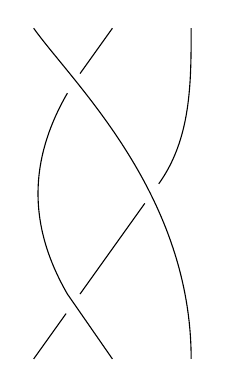
\begin{tikzpicture}
    \node[coordinate] (a0) at (0,0) {};
    \node[coordinate] (b0) at (1,0) {};
    \node[coordinate] (c0) at (2,0) {};
    \node (ab1) at (0.5,-0.7) {};
    \node (c1)  at (2,-0.7)   {};
    \node (c2)  at (2,-1.4)   {};
    \node (bc3) at (1.5,-2.1) {};
    \node (c3)  at (2,-2.1)   {};
    \node (ab5) at (0.5,-3.5) {};
    \node[coordinate] (a6) at (0,-4.2) {};
    \node[coordinate] (b6) at (1,-4.2) {};
    \node[coordinate] (c6) at (2,-4.2) {};
    
    \draw (a0) .. controls (ab1) and (c3) .. (c6);
    \draw (b0) to (ab1) to [bend right] (ab5) to (b6);
    \draw (c0) .. controls (c1) and (c2) .. (bc3)
          (bc3) to (ab5) (ab5) to (a6);
\end{tikzpicture}
\quad \raisebox{2.1cm}{=} \quad
\begin{tikzpicture}
    \node (bc1) at (1.5,-0.7) {};
    \node (a3)  at (0,-2.1)   {};
    \node (ab3) at (0.5,-2.1) {};
    \node (a4)  at (0,-2.8)   {};
    \node (a5)  at (0,-3.5)   {};
    \node (bc5) at (1.5,-3.5) {};
    
    \draw (c6) .. controls (bc5) and (a3) .. (a0);
    \draw (b6) to (bc5) to [bend right] (bc1) to (b0);
    \draw (a6) .. controls (a5) and (a4) .. (ab3)
          (ab3) to (bc1) (bc1) to (c0);
\end{tikzpicture}
\]

I won't try to draw the corresponding movie move, but just as the 3rd Reidemeister move is the basis for the Yang--Baxter equation $R_{23}R_{13}R_{12} = R_{12}R_{13}R_{23}$ (the subscripts indicate which strand is crossing which), the corresponding movie move is the basis for a variant of the ``Frenkel--Moore'' form of the ``Zamolodchikov tetrahedron equation'' which first arose in string theory. This variant goes like: $S_{124}S_{135}S_{236}S_{456} = S_{456}S_{236}S_{135}S_{124}$ and Carter and Saito draw pictures that make this equation almost as obvious as the Yang--Baxter equations.

In any event, this is becoming a very hot subject, since topologists are interested in generalizing the new results on knot theory to higher dimensions, while some physicists (especially Louis Crane) are convinced that this is the right way to tackle the ``problem of time'' in quantum gravity (which, in the loop variables approach, amounts to studying the relationship of knot theory to the 4th dimension, time.) In particular, Carter and Saito are investigating how to construct solutions of the Zamolodchikov equations from solutions of the Yang--Baxter equation - the goal presumably being to find invariants of knotted surfaces that are closely related to the link invariants coming from quantum groups. This looks promising, since Crane and Yetter have just constructed a 4-dimensional topological quantum field theory from the quantum SU(2). But apparently nobody has yet done it.

Lovers of category theory will be pleased to learn that the correct framework for this problem appears to be the theory of 2-categories. These are categories with objects, morphisms between objects, and also ``2-morphisms'' between objects. The idea is simply that tangles are morphisms between sets of points (i.e., each of the tangles in the picture above are morphisms from 3 points to 3 points), while surfaces in $\R^4$ are 2-morphisms between tangles. The instigators of the 2-categorical approach here seem to be Kapranov and Voevodsky, whose paper ``2-categories and Zamolodhikov tetrahedra equations,'' to appear in Proc. Symp. in Pure Math., is something I will have to get ahold of soon by any means possible (I can probably nab it from Oleg Viro down the hall; he is currently hosting Kharmalov, who is giving a series of talks on knotted surfaces at 2-categories here at UCR.) But it seems to be Louis Crane who is most strongly proclaiming the importance of 2-categories in \emph{physics}.

\find{\paper{Knot theory and quantum gravity in loop space: a primer, by Jorge Pullin, to appear in ``Proc. of the Vth Mexican School of Particles and Fields,'' ed. J. L. Lucio, World Scientific, Singapore, now available as \href{https://arxiv.org/abs/hep-th/9301028}{arXiv:hep-th/9301028}.}}

This is a review of the new work on knot theory and the loop representation of quantum gravity. Pullin is among a group who has been carefully studying the ``Chern--Simons state'' of quantum gravity, so his presentation, which starts with a nice treatment of the basics, leads towards the study of the Chern--Simons state. This is by far the best-understood state of quantum gravity, and is defined by SU(2) Chern--Simons theory in terms of the connection representation, or by the Kauffman bracket invariant of knots in the loop representation. It is a state of Euclideanized quantum gravity with nonzero cosmological constant, and is not invariant under CP. Ashtekar has recently speculated that it is a kind of ``ground state'' for gravity with cosmological constant (evidence for this has been given by Kodama), and that its CP violation may be a ``reason'' for why the cosmological constant is actually zero (this part is extremely speculative). Louis Crane, on the other hand, seems convinced that the Chern--Simons state (or more generally states arising from modular tensor categories) is THE WAVEFUNCTION OF THE UNIVERSE. In any event, it's much nicer to have one state of quantum gravity to play with than none, as was the case until recently.

\find{\paper{Time, measurement and information loss in quantum cosmology, by Lee Smolin, preprint now available as \href{https://arxiv.org/abs/gr-qc/9301016}{arXiv:gr-qc/9301016}.}}

This is, as usual for Smolin, a very ambitious paper. It attempts to sketch a solution of some aspects of the problem of time in quantum gravity (in terms of the loop representation). I might as well quote from the introduction:

Thus, to return to the opening question, if we are, within a nonperturbative framework, to ask what happens after a black hole evaporates, we must be able to construct spacetime diffeomorphism invariant operators that can give physical meaning to the notion of ``after the evaporation.'' Perhaps I can put it in the following way: the questions about loss of information or breakdown of unitary evolution rely, implicitly, on a notion of time. Without reference to time it is impossible to say that something is being lost. In a quantum theory of gravity, time is a problematic concept which makes it difficult to even ask such questions at the nonperturbative level, without reference to a fixed spacetime manifold. [I would prefer to say ``fixed background metric'' - JB] The main idea, which it is the purpose of this paper to develop, is that the problem of time in the nonperturbative framework is more than an obstacle that blocks any easy approach to the problem of loss of information in black hole evaporation. It may be the key to its solution.

As many people have argued, the problem of time is indeed the conceptual core of the problem of quantum gravity. Time, as it is conceived in quantum mechanics is a rather different thing than it is from the point of view of general relativity. The problem of quantum gravity, especially when put in the cosmological context, requires for its solution that some single concept of time be invented that is compatible with both diffeomorphism invariance and the principle of superposition. However, looking beyond this, what is at stake in quantum gravity is indeed no less and no more than the entire and ancient mystery: What is time? For the theory that will emerge from the search for quantum gravity is likely to be the background for future discussions about the nature of time, as Newtonian physics has loomed over any discussion about time from the seventeenth century to the present.

I certainly do not know the solution to the problem of time. Elsewhere I have speculated about the direction in which we might search for its ultimate resolution. In this paper I will take a rather different point of view, which is based on a retreat to what both Einstein and Bohr taught us to do when the meaning of a physical concept becomes confused: reach for an operational definition. Thus, in this paper I will adopt the point of view that time is precisely no more and no less than that which is measured by physical clocks. From this point of view, if we want to understand what time is in quantum gravity then we must construct a description of a physical clock living inside a relativistic quantum mechanical universe.

Technically speaking, what Smolin does is roughly as follows. He considers quantum gravity coupled to matter, modelled in such a way that the Hilbert space is spanned by states labelled by isotopy classes of: any number N loops in a compact 3-manifold M (``space'') and N surfaces with boundary in M. (This trick is something I hadn't seen before, though Smolin gives references to it.) He then introduces a ``clock field,'' which is just a free scalar field coupled to the gravity, and does gauge-fixing to see what evolution with respect to this clock field looks like. I will have to read this a number of times!
